Qui, di seguito, viene riportata l'architettura relativa alla seconda solution.

\lstinputlisting[language=C++]{solutions/s2/s2.cpp}

In particolare, nella soluzione hardware in questione, rispetto alla solution 1, è stato aggiunto la direttiva di pipeline all'interno del loop2. Pertanto, ci si dovrebbe aspettare una minore latenza totale dal momento che il pipelining permette di scindere le operazioni complesse in più operazioni semplici. In questo modo si può far lavorare l’architettura con dati temporalmente differenti. 

\begin{figure}[H]
	\centering
	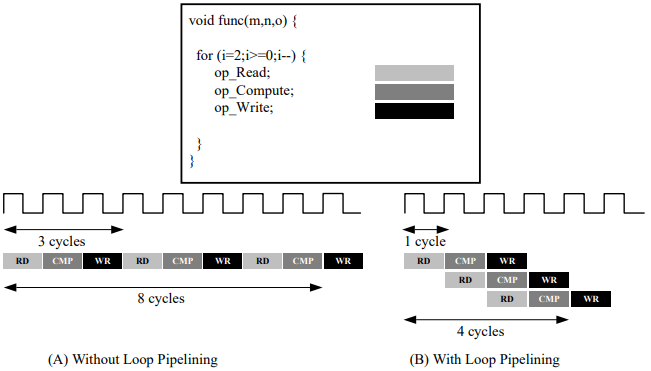
\includegraphics[width=0.5\textwidth]{solutions/s2/looppipelining.png}
	\caption{HLS Loop Pipelining}
\end{figure}

Effettuando la sintesi è possibile evidenziare il seguente report:\\

\begin{table}[H]
	\centering
	\begin{minipage}[t]{0.45\linewidth}
		\centering
		\begin{tabular}{|c|c|c|c|}
			\hline
			\textbf{Clock} & \textbf{Target} & \textbf{Estimated} & \textbf{Uncertainty} \\
			\hline
			ap\_clk & 10.00 & 8.510 & 1.25 \\
			\hline
		\end{tabular}
		\caption{HLS Solution 2 Timing Summary (ns)}
		\label{tab:hls-solution-2-timing-summary}
	\end{minipage}
	\hfill
	\begin{minipage}[t]{0.45\linewidth}
		\centering
		\begin{tabular}{|c|c|c|c|}
			\hline
			\multicolumn{2}{|c|}{\textbf{Latency}} & \multicolumn{2}{|c|}{\textbf{Interval}} \\
			min & max & min & max \\
			\hline
			17 & 45 & 17 & 45 \\
			\hline
		\end{tabular}
		\caption{HLS Solution 2 Latency Summary (clock cycles)}
		\label{tab:hls-solution-2-latency-summary}
	\end{minipage}
\end{table}

\begin{table}[H]
	\centering
	\begin{tabular}{|c|c|c|c|c|c|c|c|c|}
		\hline
		\multicolumn{1}{|c|}{Loop} & \multicolumn{2}{|c|}{\textbf{Latency}} & \multicolumn{1}{c|}{\textbf{Iteration Latency}} & \multicolumn{2}{c|}{\textbf{Initiation Interval}} & \multicolumn{1}{c|}{\textbf{Trip Count}}  \\
		Name & min & max &  & achieved & target &  \\
		\hline
		- loop1 & 16 & 44 & 4$\sim$11 & - & - & 4 \\
		+ loop2 & 0 & 7 & 5 & 1 & 1 & 0$\sim$4 \\
		\hline
	\end{tabular}
	\caption{HLS Solution 2 Latency Loops Summary}
	\label{tab:hls-solution-2-loop-summary}
\end{table}

Si può notare, rispetto alla solution precedente, come in questo caso venga specificato un valore numerico di Initiation Interval (II). In particolare, l'II\_achieved risulta essere il medesimo di quello target, cioè uguale a 1. Teoricamente, come in questo caso, si dovrebbe ottenere II\_target=II\_achieved. Se così non fosse allora il tool non è riuscito a raggiungere l'obiettivo prefissato e si dovrebbero attuare modifiche all'architetture o caso mai prevedere l'utilizzo di ulteriori direttive.
\\
Qui di seguito, viene allegato l'utilizzazione delle risorse stimata dal processo di sintesi.
\begin{table}[H]
	\centering
	\begin{tabular}{|l|c|c|c|c|}
		\hline
		\textbf{Name}    & \textbf{BRAM\_18K} & \textbf{DSP48E} & \textbf{FF} & \textbf{LUT} \\ \hline
		DSP              & -                   & -               & -           & -            \\ 
		Expression       & -                   & 3               & 0           & 141          \\ 
		FIFO             & -                   & -               & -           & -            \\ 
		Instance         & -                   & -               & -           & -            \\ 
		Memory           & 0                   & -               & -          & -            \\ 
		Multiplexer      & -                   & -               & -           & 78          \\ 
		Register         & -                   & -               & 340         & 32            \\ \hline
		\textbf{Total}   & 0                   & 3               & 340         & 251          \\ \hline
		\textbf{Available} & 280               & 220             & 106400      & 53200        \\ \hline
		\textbf{Utilization (\%)} & 0            & 1               & $\sim$0     & $\sim$0      \\ \hline
	\end{tabular}
	\caption{HLS Solution 2 Utilization Estimates Summary}
	\label{tab:hls-solution-2-utilization-estimates-summary}
\end{table}

Successivamente effettuando la C/RTL Cosimulation e l'Export RTL è possibile evidenziare i seguenti report.
\begin{table}[H]
	\centering
	\begin{tabular}{|c|c|c|c|c|c|c|c|}
		\hline
		\multicolumn{1}{|c|}{RTL} & \multicolumn{1}{|c|}{Status} & \multicolumn{3}{c|}{\textbf{Latency}} & \multicolumn{3}{c|}{\textbf{Interval}} \\
		&  & min & avg & max & min & avg & max \\
		\hline
		VHDL & Pass & 38 & 38 & 38 & NA & NA & NA \\
		\hline
	\end{tabular}
	\caption{HLS Solution 1 with Trip Count C/RTL Cosimulation Summary }
	\label{tab:hls-solution-1-cosimulation-summary}
\end{table}

In particolare, si può notare come, in seguito all'introduzione della direttiva di pipeline, il numero di risorse risulta essere cambiato. Nello specifico, l'utilizzazione delle LUT è aumentata di circa il $24\%$ mentre quella dei FF è diminuita di circa il $14\%$.

\begin{table}[H]
	\centering
	\begin{minipage}[t]{0.45\linewidth}
		\centering
		\begin{tabular}{|l|r|}
			\hline
			\textbf{Resource} & \textbf{VHDL} \\
			\hline
			SLICE & 38 \\
			\hline
			LUT & 115 \\
			\hline
			FF & 139 \\
			\hline
			DSP & 3 \\
			\hline
			BRAM & 0 \\
			\hline
			SRL & 0 \\
			\hline
		\end{tabular}
		\caption{HLS Solution 2t Export RTL Resource Usage}
		\label{tab:hls-solution-2-export-rtl-resoruce-usage}
	\end{minipage}
	\hfill
	\begin{minipage}[t]{0.45\linewidth}
		\centering
		\begin{tabular}{|l|r|}
			\hline
			\textbf{Timing} & \textbf{VHDL} \\
			\hline
			CP required & 10.000 \\
			\hline
			CP achieved post-synthesis & 5.745 \\
			\hline
			CP achieved post-implementation & 5.718 \\
			\hline
		\end{tabular}
		\caption{HLS Solution 2 Export RTL Final Timing}
		\label{tab:hls-solution-2-export-rtl-final-timing}
	\end{minipage}
\end{table}